\documentclass{ximera}

\input{../preamble.tex}

\outcome{Know the properties of rational functions.}
\outcome{Understand the definition of a rational function.}

\title[Dig-In:]{Working with rational functions}


\begin{document}
\begin{abstract}
  Rational functions are functions defined by fractions of
  polynomials.
\end{abstract}
\maketitle


\section{What are rational functions?}
In algebra, polynomials play the same role as the integers do in arithmetic.  We add them, subtract them, multiply them, and factor them.  We cannot 
divide them, however, if we want an integer answer.  Since $4$ is not a factor of $7$, $\dfrac{7}{4}$ is not an integer.  If we want to be able to divide
integers, we have to move to the \emph{rational numbers}, which are fractions $\dfrac{p}{q}$ where $p$ and $q$ are integers, and $q \ne 0$.

The same idea holds for polynomials.  We can add them, subtract them, multiply them, and factor them.  However, to divide them we have to move
to rational functions.

\begin{definition}
  A \dfn{rational function} in the variable $x$ is a function the form
  \[
  f(x) = \frac{p(x)}{q(x)}
  \]
  where $p$ and $q$ are polynomial functions, and $q$ is not the constant zero function. The domain of a rational
  function is all real numbers except for where the denominator is
  equal to zero.
\end{definition}

\begin{question}
  Which of the following are rational functions?
  \begin{selectAll}
    \choice[correct]{$f(x) = 0$}
    \choice[correct]{$f(x) = \frac{3x+1}{x^2-4x+5}$}
    \choice{$f(x)=e^x$}
    \choice{$f(x)=\frac{\sin(x)}{\cos(x)}$}
    \choice[correct]{$f(x) = -4x^{-3}+5x^{-1}+7-18x^2$}
    \choice{$f(x) = x^{1/2}-x +8$}
    \choice{$f(x)=\frac{\sqrt{x}}{x^3-x}$}
  \end{selectAll}
  \begin{feedback}
    All polynomials can be thought of as rational functions.
  \end{feedback}
\end{question}



\section{Working with rational functions}

\begin{example}
	Find the domain of the rational function $\displaystyle f(x) = \dfrac{4x^3+1}{6x^2-7x-3}$
	\begin{explanation}
		We start by setting the denominator equal to zero.
		\begin{align*}
			6x^2 - 7x - 3 &= 0\\
			(3x + 1)(2x - 3)&= 0\\
			x &= -\dfrac{1}{3} , \dfrac{3}{2}
		\end{align*}
		The domain of $f$ is all $x$ except these two values.  Thus:
		\[ \left( -\infty , \dfrac{1}{3}\right) \bigcup \left( -\dfrac{1}{2}, \dfrac{3}{2} \right) \bigcup \left( \dfrac{3}{2}, \infty \right). \]
	\end{explanation}
\end{example}


When we need to simplify the form of a rational expression, our approach depends on the particular form we are presented with.  If it consists of
only a single fraction, we divide out the common factors.
\begin{example}
	Simplify the expression $\displaystyle \dfrac{2x^2-3x-2}{4x^2+6x+2}$.
	\begin{explanation}
		We begin by factoring.  The numerator factors as $2x^2 - 3x -2 = (2x+1)(x-2)$, and the denominator factors as $4x^2+6x+2 = 2(2x+1)(x+1)$.
		That means,
		\begin{align*}
			\dfrac{2x^2-3x-2}{4x^2 + 6x + 2} &= \dfrac{(2x+1)(x-2)}{2(2x+1)(x+1)} \\
				&= \dfrac{2x+1}{2x+1} \cdot \dfrac{x-2}{2(x+1)}\\
				&= \dfrac{x-2}{2(x+1)},
		\end{align*}	
		where we used the fact that $\displaystyle \dfrac{2x+1}{2x+1} = 1$.
	\end{explanation}
\end{example}

When dealing with a sum/difference of two fractions, we must first convert to a common denominator.  After the addition,
we can divide away any common factors that are still present.
\begin{example}
	Simplify the expression \[ \dfrac{x-6}{x^2+2x} + \dfrac{x+3}{x^2+x}. \]
	\begin{explanation}
		We'll start by factoring the denominators.  $x^2+2x = x(x+2)$, and $x^2+x = x(x+1)$.
		These two fractions have a common denominator of $x(x+1)(x+2)$.
		\begin{align*}
			\dfrac{x-6}{x^2+2x} + \dfrac{x+3}{x^2+x} &= \dfrac{x-6}{x(x+2)} + \dfrac{x+3}{x(x+1)}\\
				&= \dfrac{(x-6)(x+1)}{x(x+2)(x+1)} + \dfrac{(x+3)(x+2)}{x(x+1)(x+2)}\\
				&= \dfrac{x^2-5x-6}{x(x+2)(x+1)} + \dfrac{x^2+5x+6}{x(x+2)(x+1)}\\ 
				&= \dfrac{2x^2}{x(x+2)(x+1)}\\
				&= \dfrac{2x}{(x+2)(x+1)}.
		\end{align*}
		Once we convert each fraction to the common denominator, we added numerators, then simplified.
	\end{explanation}
\end{example}

If we have a complex fraction, involving a fraction in the numerator or the denominator, we can start by multiplying the numerator
and denominator of the big fraction, by the common denominator of the smaller fractions.  That eliminates the smaller fractions leaving
the outer one to deal with.
\begin{example}
	Simplify the expression \[ \dfrac{ \dfrac{x+2}{x-1} + x}{\dfrac{x}{x-1} + \dfrac{2x+1}{x+1}}.\]
	\begin{explanation}
		The smaller fractions in the numerator and denominator have a common denominator $(x-1)(x+1)$.  We begin my multiplying
		both the numerator and denominator by $(x-1)(x+1)$.
		\begin{align*}
			\dfrac{ \dfrac{x+2}{x-1} + x}{\dfrac{x}{x-1} + \dfrac{2x+1}{x+1}} &= \dfrac{ \dfrac{x+2}{x-1} + x}{\dfrac{x}{x-1} + \dfrac{2x+1}{x+1}} \cdot \dfrac{(x-1)(x+1)}{(x-1)(x+1)}\\
				&= \dfrac{(x+2)(x+1) + x(x+1)(x-1)}{x(x+1) + (2x+1)(x-1)}\\
				&= \dfrac{(x+1)\left( (x+2)  + (x^2-x) \right)}{(x^2+x) + (2x^2 - x - 1)}\\
				&= \dfrac{(x+1)\left( x^2 + 2 \right)}{3 x^2 - 1}
		\end{align*}
		There are no common factors between the numerator and denominator, so this cannot be simplified any further.
	\end{explanation}
\end{example}

\begin{example}
	For the rational function $\displaystyle f(x) = \frac{2x}{x-3}$, find and simplify the following:
		\[ \frac{f(x+h)-f(x)}{h} \]
	\begin{explanation}
		$\displaystyle f(x+h)$ means replace $x$ in the formula for $f$ with $x+h$.  This gives:
		\begin{align*}
			\frac{\frac{2(x+h)}{(x+h)-3} - \frac{2x}{x-3} }{h} &= \frac{ \frac{2x+2h}{x+h-3} - \frac{2x}{x-3}}{h} \\
				&= \frac{ \frac{ (2x+2h)(x-3) }{(x+h-3)(x-3)} - \frac{2x(x+h-3)}{(x-3)(x+h-3)} }{h}\\
				&= \frac{ \frac{2x^2-6x+2xh-6h}{(x+h-3)(x-3)} - \frac{2x^2+2xh-6x}{(x+h-3)(x-3)}  }{h}\\
				&= \frac{  \frac{-6h}{(x+h-3)(x-3)}     }{h} \\
				&= \frac{-6h}{h(x+h-3)(x-3)} \\
				&= \frac{-6}{(x+h-3)(x-3)}.
		\end{align*}
	\end{explanation}
\end{example}


To solve equations involving rational expressions, we have the freedom to clear out fractions before proceeding.
After multiplying both sides by the common denominator, we are left with a polynomial equation.
\begin{example}
	Solve the equation
	\[  \frac{2}{x} + \frac{3x}{x+1} = 4.\]
	\begin{explanation}
		The common denominator is $x(x+1)$.  We multiply both sides by $x(x+1)$ to clear out the fractions.
		\begin{align*}
			\frac{2}{x} + \frac{3x}{x+1} &= 4	\\
			x(x+1) \left( \frac{2}{x} + \frac{3x}{x+1} \right) &= x(x+1) ( 4 )\\
			x(x+1) \cdot \frac{2}{x}  + x(x+1) \cdot \frac{3x}{x+1} &= 4x(x+1)\\
			2(x+1) + 3x(x) &= 4x^2 + 4x\\
			3x^2 + 2x + 2 &= 4x^2 + 4x\\
			x^2 + 2x - 2 &= 0.
		\end{align*}
		The quadratic formula gives solutions as $\displaystyle x = \dfrac{-2 \pm \sqrt{12}}{2} = -1 \pm \sqrt{3}$.
		
		If we look back at the original equation, we notice that there are some numbers that we are not allowed to plug in for $x$.  When $x=0$ or $x=-1$,
		the left-hand side of the equation is not defined due to a division by zero issue.  Since neither $-1 + \sqrt{3}$ nor $-1-\sqrt{3}$ have such an issue,
		they are both solutions.
	\end{explanation}
\end{example}

\begin{question}
	One solution of the equation \[ \dfrac{2}{x+1}+ \dfrac{1}{x+2} = 1 \] is $x = \sqrt{3}$.  Find another solution. 
	\begin{prompt}
		\[ x = \answer{-\sqrt{3}} \]
	\end{prompt}
\end{question}

\section{Inequalities}
When faced with nonlinear inequalities, such as those involving general rational functions, we make use of a sign chart.
The inequality in the following example is not given in factored form, so we have some work to do.
\begin{example}
	Solve the inequality $\displaystyle x^2 + 5x \leq -10 -\dfrac{16}{x-2}$.
	\begin{explanation}
		We'll begin by moving everything to one side, then combining them all together into a single fraction.
		\begin{align*}
			x^2 + 5x &\leq -10 -\dfrac{16}{x-2}\\
			x^2 + 5x +10 +\dfrac{16}{x-2} &\leq 0\\
			\left(x^2+5x+10\right) \cdot \left(\dfrac{x-2}{x-2}\right) +\dfrac{16}{x-2} &\leq 0\\
			\dfrac{x^3+3x^2-20}{x-2} + \dfrac{16}{x-2} &\leq 0\\
			\dfrac{x^3+3x^2-4}{x-2} &\leq 0\\
			\dfrac{(x-1)(x+2)^2}{x-2} &\leq 0
		\end{align*}
		Now that the inequality is in a better form for us to work with, we'll build a sign chart like we did in the last example.

		\begin{tikzpicture} 
			\tkzTabInit[lgt=2,espcl=1] 
				{$x$         /1, 
				$x-1$   /1, 
				$\left(x+2\right)^2$  /1,
				$x-2$       /1}% 
				{  , $-2$ , $1$ ,$2$,  }% 
			\tkzTabLine{ , - , t , - , t , + , d , + ,}
			\tkzTabLine{ , + , t , + , t , + , d , + ,}
			\tkzTabLine{ , - , t , - , t , - , d , +, }
		\end{tikzpicture} 

		We see from the chart that $\displaystyle \dfrac{(x-1)(x+2)^2}{x-2}$ will be negative in $(1,2)$.  At $x=-2$ and $x=1$ it is zero.
		The solution is then: $\left\{ -2\right\} \cup [ 1, 2 )$.
	\end{explanation}
\end{example}


\begin{problem}
	Find the solution of the inequality: $\displaystyle x + \dfrac{9}{x-1} > 5$.
	\begin{multipleChoice}
		\choice{$(-1, \infty)$}
		\choice{$[-1,\infty)$}
		\choice[correct]{$(-1,2)\cup (2,\infty)$}
		\choice{$\{-1\} \cup [2,\infty)$}
		\choice{none of the above}
	\end{multipleChoice}
\end{problem}


\begin{example}
	Solve the inequality
	\[ \frac{1}{x-2} - \frac{4}{x+1} \leq 3 \]
	\begin{explanation}
		We'll start by moving everything to the left-hand side and combining them into a single fraction.
		\begin{align*}
			\frac{1}{x-2} - \frac{4}{x+1} &\leq 3 \\
			\frac{1}{x-2} - \frac{4}{x+1} - 3 &\leq 0\\
			\frac{1(x+1)}{(x-2)(x+1)} - \frac{4(x-2)}{(x+1)(x-2)} - \frac{3(x+1)(x-2)}{(x+1)(x-2)} &\leq 0\\
			\frac{(x+1) - (4x-8) - (3x^2-3x-6)}{(x+1)(x-2)} &\leq 0\\
			\frac{-3x^2+15}{(x+1)(x-2)} &\leq 0\\
			\frac{-3(x^2-5)}{(x+1)(x-2)} &\leq 0
		\end{align*}
		To solve this, we'll construct a sign chart.  We start by noticing that $x^2-5 =0$ only if $x = \pm \sqrt{5}$.
		\begin{tikzpicture} 
			\tkzTabInit[lgt=2,espcl=1] 
				{$x$         /1, 
				$-3$    /1,
				$x^2-5$   /1, 
				$x+1$  /1,
				$x-2$       /1}% 
				{  , $-\sqrt{5}$ , $-1$ , $2$, $\sqrt{5}$,   }% 
			\tkzTabLine{ , - , t , - , d , - , d , - , t, -, }
			\tkzTabLine{ , + , t , - , d , - , d , - , t, +,}
			\tkzTabLine{ , - , t , - , d , + , d , +, t, +, }
			\tkzTabLine{ , - , t , - , d , - , d , +, t, +, }
		\end{tikzpicture} 
		
		We see from the sign chart, that the solution is $\displaystyle \left( -\infty, -\sqrt{5} \right] \bigcup \left(-1, 2\right) \bigcup \left[ \sqrt{5}, \infty \right)$.
	\end{explanation}
\end{example}







\section{What can the graphs look like?}

There is a somewhat wide variation in the graphs of rational
functions.

\begin{example}
    Here we see the the graphs of four rational functions.
\begin{image}
  \begin{tabular}{cc}
    \begin{tikzpicture}
      \begin{axis}[
          xmin=-30,xmax=30,
            ymin=-30,ymax=30,
            domain=-2:2,
            width=2.5in,
            axis lines =middle, xlabel=$x$, ylabel=$y$,
            every axis y label/.style={at=(current axis.above origin),anchor=south},
            every axis x label/.style={at=(current axis.right of origin),anchor=west},
        ]
	\addplot [very thick, penColor, smooth, samples=100, domain=-30:-2.2] {(x^2-3*x+2)/(x+2)};
       	\addplot [very thick, penColor, smooth, samples=100, domain=-1.8:30] {(x^2-3*x+2)/(x+2)};

        \node at (axis cs:10,15) [penColor,anchor=west] {$A$};          
      \end{axis}
    \end{tikzpicture}
    &
    \begin{tikzpicture}
	\begin{axis}[
            xmin=-2,xmax=4,
            ymin=-3,ymax=3,
            width=2.5in,
            axis lines =middle, xlabel=$x$, ylabel=$y$,
            every axis y label/.style={at=(current axis.above origin),anchor=south},
            every axis x label/.style={at=(current axis.right of origin),anchor=west},
          ]
	  \addplot [very thick, penColor2, domain=-2:.9] {1/(x-1)};
          \addplot [very thick, penColor2, domain=1.1:4] {1/(x-1)};
          \addplot[color=penColor2,fill=background,only marks,mark=*] coordinates{(2,1)};  %% open hole
          \node at (axis cs:2.5,1.3) [penColor2] {$B$};
        \end{axis}
    \end{tikzpicture}
        \\
    \begin{tikzpicture}
      \begin{axis}[
          xmin=-1,xmax=5,
          ymin=-30,ymax=30,
          width=2.5in,
          axis lines =middle, xlabel=$x$, ylabel=$y$,
          every axis y label/.style={at=(current axis.above origin),anchor=south},
          every axis x label/.style={at=(current axis.right of origin),anchor=west},
        ]
        \addplot [very thick, penColor3, smooth, samples=100, domain=-1:.95] {(x+2)/(x^2-3*x+2)};
        \addplot [very thick, penColor3, smooth, samples=100, domain=1.1:1.9]  {(x+2)/(x^2-3*x+2)};
        \addplot [very thick, penColor3, smooth, samples=100, domain=2.1:5]  {(x+2)/(x^2-3*x+2)};
        \node at (axis cs:3,7) [penColor3] {$C$};
      \end{axis}
    \end{tikzpicture}
    &
 \begin{tikzpicture}
      \begin{axis}[
          xmin=-2,xmax=4,
          ymin=-3,ymax=3,
          domain=-2:4,
          width=2.5in,
          axis lines =middle, xlabel=$x$, ylabel=$y$,
          every axis y label/.style={at=(current axis.above origin),anchor=south},
          every axis x label/.style={at=(current axis.right of origin),anchor=west},
        ]
	\addplot [very thick, penColor4] {x-1};
        \addplot[color=penColor4,fill=background,only marks,mark=*] coordinates{(2,1)};  %% open hole
        \node at (axis cs:3,1.5) [penColor4] {$D$};
      \end{axis}
    \end{tikzpicture}
  \end{tabular}
\end{image}
Match the curves $A$, $B$, $C$, and $D$ with the functions
  \begin{align*}
    &\frac{x^2-3x+2}{x-2}, &&\frac{x^2-3x+2}{x+2}, \\
    &\frac{x-2}{x^2-3x+2}, &&\frac{x+2}{x^2-3x+2}.
  \end{align*}
\begin{explanation}
  Consider $\frac{x^2-3x+2}{x-2}$. This function is undefined only at
  $x=2$. Of the curves that we see above, $\answer[given]{D}$ is
  undefined exactly at $x=2$.

  Now consider $\frac{x^2-3x+2}{x+2}$. This function is undefined only
  at $x=-2$. The only function above that undefined exactly at $x=-2$
  is curve $\answer[given]{A}$.

  Now consider $\frac{x-2}{x^2-3x+2}$. This function is undefined at
  the roots of
  \[
  x^2-3x+2 = (x-2)(x-1).
  \]
  Hence it is undefined at $x=2$ and $x=1$. It looks like both curves
  $B$ and $C$ would work. Distinguishing between these two curves is
  easy enough if we evaluate at $x=-2$. Check it out.
  \begin{align*}
    \eval{\frac{x-2}{x^2-3x+2}}_{x=-2} &= \frac{-2-2}{(-2)^2-3(-2)+2}\\
    &= \frac{-4}{4+6+2}\\
    &=\frac{-4}{12}.
  \end{align*}
  Since this is negative, we see that $\frac{x-2}{x^2-3x+2}$
  corresponds to curve $\answer[given]{B}$.

  Finally, it must be the case that curve $\answer[given]{C}$
  corresponds to $\frac{x+2}{x^2-3x+2}$. We should note that if this
  function is evaluated at $x=-2$, the output is zero, and this
  corroborates our work above.
\end{explanation}
\end{example}


%% \section{Connections to polynomials}
%% $\frac{x^2-3x+2}{x-2} \ne x-1$

\end{document}
